\documentclass{article}
\usepackage{titlesec}
\usepackage{colortbl}
\usepackage{graphicx}
\usepackage{tabularx}
\usepackage{amsmath}
\usepackage[]{algorithm2e}
\usepackage{centernot}
\usepackage{tikz}
\usetikzlibrary{shapes,arrows}
\usepackage{float}
\usepackage[utf8]{inputenc}

\title{Assignment T3. Time and Global state \\
\large TDT4190 - Distributed Systems, spring 2014}

\author{
    Sigve Sebastian Farstad \\
    Christoffer Tønnessen
}

\renewcommand\thesubsection{\alph{subsection})}
\newcommand{\question}[1]{\subsection{}\textit{#1}\bigskip}
\newcommand{\singlequestion}[1]{\textit{#1}\bigskip}
\newcommand{\answer}{\paragraph{Answer}}

\begin{document}

\maketitle

\section{Time}

\question{Why do we need both physical and logical clocks in distributed systems? Give two examples of the use of physical and logical clocks.}

\answer
Synchronized physical clocks in a distributed system are clocks that are synchronized with each other, and also with an external authorative absolute time source such as UTC.
Physical clocks are local to each node in a distributed system, and each physical clock may have a different drift and offset from the absolute time source.
This means that physical clocks are vulnerable to desynchronization due to clock skew, which can cause problems.

Physical clocks are used when a synchronized, absolute clock is needed.

Synchronized logical clocks are not synchronized with an external authoritive time source.
In a system using logical clocks, the exact time of an event is not important. Rather, only the relative partial temporal ordering of events is of interest.

Logical clocks are used when a synchronized, not-necessarily-absolute clock is needed.

Two examples of where physical clocks can be used are timestamping of events, and absolute clock-based consistency.
Two examples of where logical clocks can be used are scheduling, and deadlock prevention.


\question{The figure below shows three processes with different events. The arrows mean sending of messages. The arrow points to the process that receives the message. Which of the following pair of events have the "happened-before" relation?
}

\textit{
\begin{itemize}
\begin{centering}
    \item{a $ \rightarrow $ j}
    \item{j $ \rightarrow $ c}
    \item{k $ \rightarrow $ u}
    \item{a $ \rightarrow $ e}
    \\
\end{centering}
\end{itemize}
}

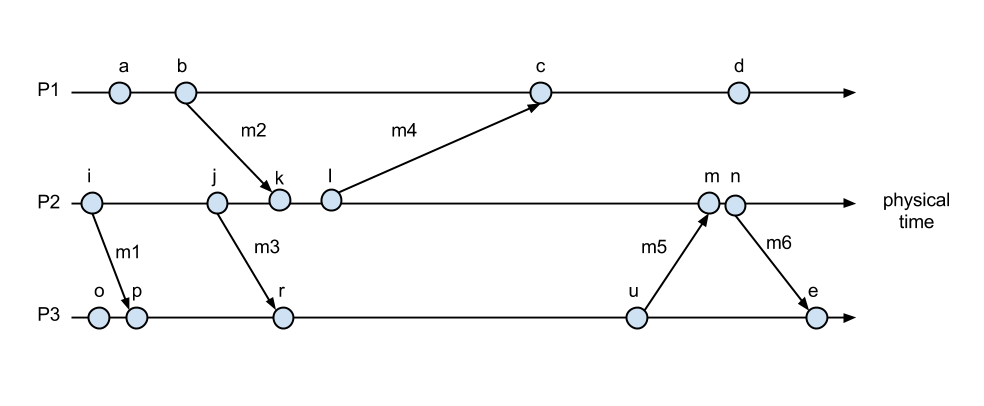
\includegraphics[width=\textwidth]{images/T3-1.png}

\answer
Happened-before is a transitive, irreflexible, antisymmetric relation.
Using the standard notation $ a \rightarrow b $ to mean $ a $ happened-before $ b$, of the four pairs of events, the following have happened-before releations:

\begin{itemize}
\begin{centering}
    \item{$ j \rightarrow c $}
    \item{$ a \rightarrow e $}
    \\
\end{centering}
\end{itemize}

\question{Given two events e and f. Assume that the logical (Lamport) clock values L are such that $L (e) < L (f)$. Can we then deduce that e "happened before" f? Why? What happens if one uses vector clocks instead? Explain.}

\answer
$ e \rightarrow f \implies L(e) < L(f) $. However, $ L(e) < L(f) \centernot\implies e \rightarrow f $.
Therefore, we must conclude that $ e $ and $ f $ are concurrent events.

Using vector clocks in each node, it is possible to infer more.
In a vector clock system with $ N $ nodes, each node keeps a vector of $ N $ clocks locally, representing the local clock of every node in the system.
Vector clocks function similar to regular logical (Lamport) clocks, except that the timestamps are vector timestamps.
Using the vector clock approach, $ a \rightarrow f \iff V(e) < V(f) $.

Therefore, if it is known that $ V(e) < V(f) $, it can be deduced that $ e \rightarrow f $.

\question{The figure below shows three processes and a number of events. Vector clock values are given for some of the events. Give the vector clock values for the remaining events.}

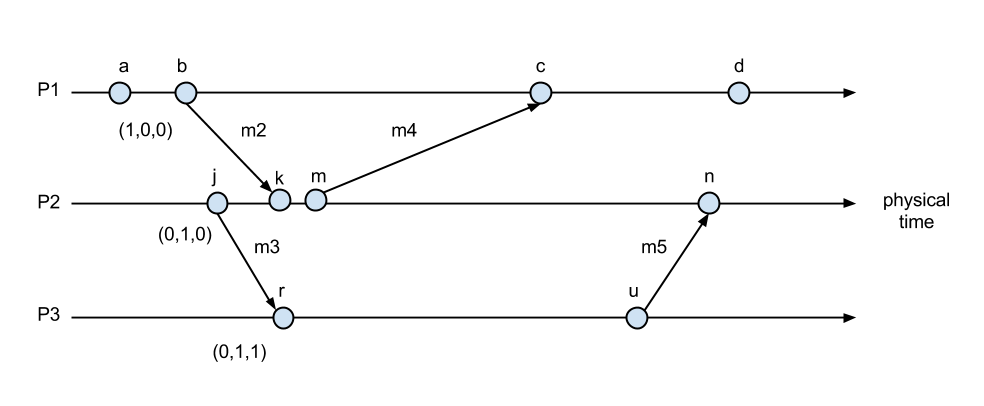
\includegraphics[width=\textwidth]{images/T3-2.png}

\answer
The vector clock values are given in table \ref{table:vector-clock-values}.

\begin{table}[H]
    \centering
    \begin{tabular}{c | c}
        Event & Vector clock value \\
        \hline
        b & (2, 0, 0) \\
        c & (3, 3, 0) \\
        d & (4, 3, 0) \\
        k & (2, 2, 0) \\
        m & (2, 3, 0) \\
        n & (2, 4, 2) \\
        u & (0, 1, 2) \\
    \end{tabular}
    \caption{Vector clock values}
    \label{table:vector-clock-values}
\end{table}

\question{A client attempts to synchronize with a time server. Timestamps comes from the server, i.e. it is the point in time that the server responds. Round trip time and timestamp are shown in the table below. Which of these timestamps should the client use to set its own clock? What time should the clock be set to? Calculate the accuracy of the new clock value with respect to the server's clock. If it turns out that the time between sending and receiving a message in the system is at least 10ms, are there any changes in your calculation?}

\answer
TODO

\section{NTP Synchronization}

\singlequestion{We want to find the difference between A's and B's clocks. B receives a message at 09:14:59.030 from A with timestamp 09:14:48.980. B sends a reply. A receives this reply at 09:15:19.425 with timestamp 09:15:09.385 (as set by B). Estimate the offset between B and A.}

\answer
With $ a $ denoting the timestamp difference between the receive-timestamp of the message received at A and the send-timestamp of that same message, and $ b $ denoting the timestamp difference between the receive-timestamp of the message received at B and the send-timestamp of that same message, the offset can be estimated to be $ \frac{a + b}{2} $, and the error can be estimated to be $ \pm \frac{a - b}{2} $.

a = 10.050
b = 10.040

Plugging the numbers, the offset is $ \frac{a + b}{2} = 10.045 $ seconds, and the error is $ \pm \frac{a - b}{2} = 0.005 $ seconds.

\section{Global State}

\singlequestion{The figure below shows the events that occur at two processes P1 and P2. The arrows mean sending of messages. Show the alternative consistent states the system can have had. Start from state $ S_{00} $. ($ S_{xy} $ where $ x $ is p1's state and $ y $ is p2's state)}

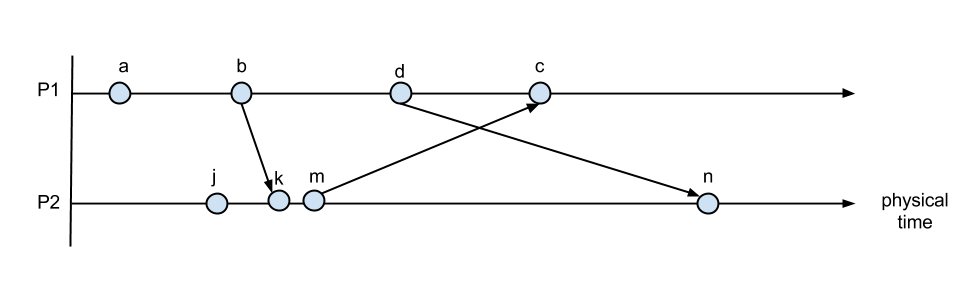
\includegraphics[width=\textwidth]{images/T3-3.png}

\answer
The alternative consistent states of the system can be seen in figure \ref{figure:alternative-consistent-states}.

\begin{figure}[H]
\tikzstyle{state} = [circle, draw, text centered]
\tikzstyle{line} = [draw, -latex']
\resizebox{\textwidth}{!}{
\begin{tikzpicture}[node distance = 1.6cm, auto]
    \tikzstyle{every node}=[font=\small]
    % Place nodes
    \node [state] (s00) {$ S_{00} $};
    \node [state, right of=s00] (s10) {$ S_{10} $};
    \node [state, right of=s10] (s20) {$ S_{20} $};
    \node [state, right of=s20] (s21) {$ S_{21} $};
    \node [state, right of=s21] (s22) {$ S_{22} $};
    \node [state, right of=s22] (s23) {$ S_{23} $};
    \node [state, right of=s23] (s33) {$ S_{33} $};
    \node [state, right of=s33] (s34) {$ S_{34} $};
    \node [state, right of=s34] (s44) {$ S_{44} $};

    \node [state, below of=s10] (s01) {$ S_{01} $};
    \node [state, below of=s20] (s11) {$ S_{11} $};
    \node [state, below of=s21] (s30) {$ S_{30} $};
    \node [state, below of=s22] (s31) {$ S_{31} $};
    \node [state, below of=s23] (s32) {$ S_{32} $};
    \node [state, below of=s34] (s43) {$ S_{43} $};
    % Draw edges
    \path [line] (s00) -- (s10);
    \path [line] (s00) -- (s01);
    \path [line] (s10) -- (s20);
    \path [line] (s10) -- (s11);
    \path [line] (s01) -- (s11);
    \path [line] (s20) -- (s21);
    \path [line] (s20) -- (s30);
    \path [line] (s11) -- (s21);
    \path [line] (s21) -- (s22);
    \path [line] (s30) -- (s31);
    \path [line] (s22) -- (s23);
    \path [line] (s22) -- (s32);
    \path [line] (s31) -- (s32);
    \path [line] (s23) -- (s33);
    \path [line] (s32) -- (s33);
    \path [line] (s33) -- (s34);
    \path [line] (s33) -- (s43);
    \path [line] (s34) -- (s44);
    \path [line] (s43) -- (s44);
\end{tikzpicture}
}
\caption{Alternative consistent states.}
\label{figure:alternative-consistent-states}
\end{figure}

                    
%s00 --> s10 --> s20 --> s21 --> s22 --> s23 --> s33 --> s34 --> s44
%    \-> s01 -\> s11 /\> s30 --> s31 -\> s32 /       \-> s43 /

\section{Snapshot}

\singlequestion{Assume two processes \textbf{A} and \textbf{B} (see figure) connected to each other by channels ($ c_1 $ and $ c_2 $) and which are sending each other a message m constantly. There are at any given time only one copy of message m in the system. Each process state consists of the number of times it has received message m, i.e., the value of the logical clock. Sending and receiving messages change the logical clock value and thus the state. Now \textbf{A} sends message m which has received state 21. Shortly after, \textbf{A} begins the snapshot algorithm. Explain which steps the algorithm consists of and the possible global state it will find in this case.}

\begin{center}
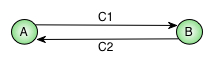
\includegraphics{images/T3-4.jpg}
\end{center}

\answer
\begin{enumerate}
    \item{\textbf{A} records its state (2).}
    \item{\textbf{A} sends a marker to \textbf{B} over $ c_1 $.}
    \item{\textbf{B} receives the marker from \textbf{A}.}
    \item{\textbf{B} records its state (22).}
    \item{\textbf{B} records the state of $ c_1 $ as null.}
    \item{\textbf{B} sends a marker to \textbf{A} over $ c2 $.}
    \item{\textbf{A} records the state of $ c2 $ as all messages received since the last time \textbf{A} recorded its state.}
\end{enumerate}

\end{document}
